\chapter{METODOLOGI PENELITIAN}
\label{chap:metodologipenelitian}

% Ubah bagian-bagian berikut dengan isi dari desain dan implementasi

Untuk mencapai tujuan dalam tugas akhir ini, dilakukan beberapa tahap yang dimulai dengan memahami fenomena \textit{ground resonance} pada helikopter melalui studi pustaka serta teori pendukung. Berikutnya adalah melakukan perumusan terhadap permasalahan yang akan diselesaikan, dalam hal ini adalah terkait dengan fenomena \textit{ground resonance} helikopter modifikasi PTDI.

Terdapat 3 pekerjaan yang dikerjaan secara paralel dan berurutan, yaitu pengukuran di tanah \textit{ground test} helikopter, perhitungan matematis secara teori dan komputasi Matlab serta simulasi menggunakan \textit{software} Femap. Sehingga bila direpresentasikan dalam bentuk alur pengerjaannya dapat dilihat pada gambar \ref{fig:TA_flow-Page-1.jpg} dan \ref{fig:TA_flow-Page-2.jpg}.
 
\begin{figure}[H]
	\centering
	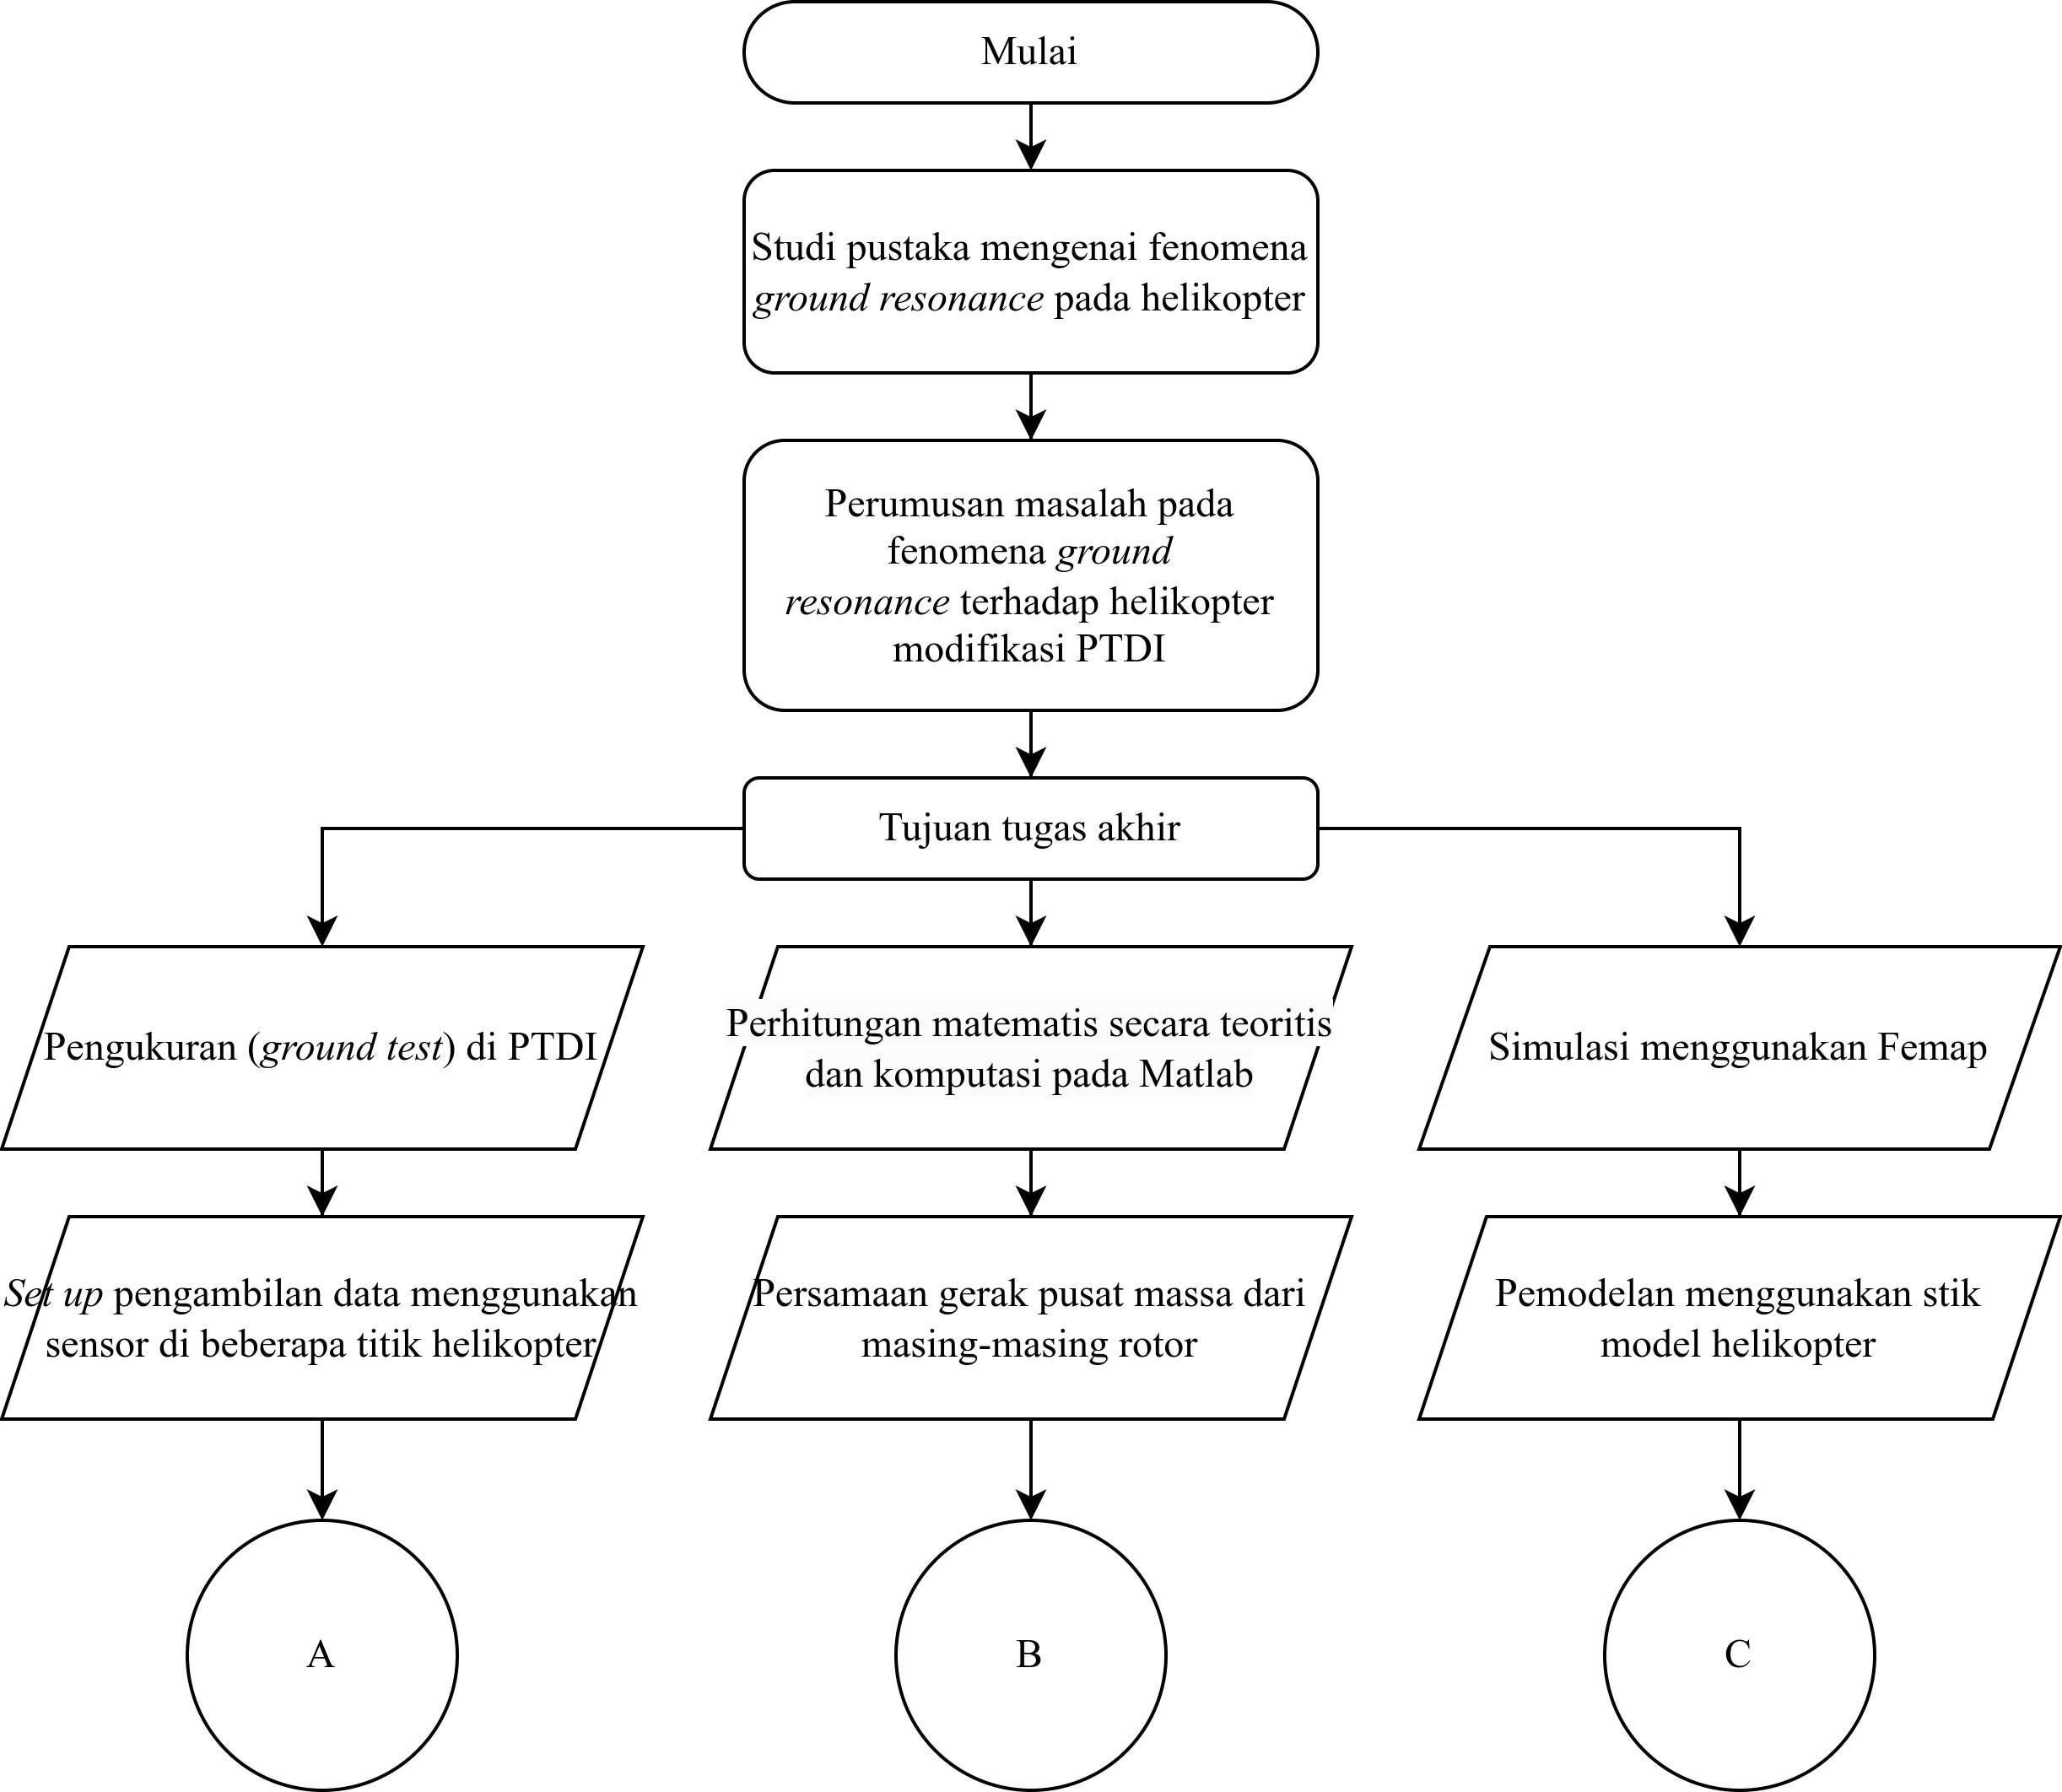
\includegraphics[width=1\linewidth]{gambar/TA_flow-Page-1.jpg}
	\caption{Diagram alir pengerjaan Tugas Akhir bagian 1.}
	\label{fig:TA_flow-Page-1.jpg}
\end{figure}

\begin{figure}[H]
	\centering
	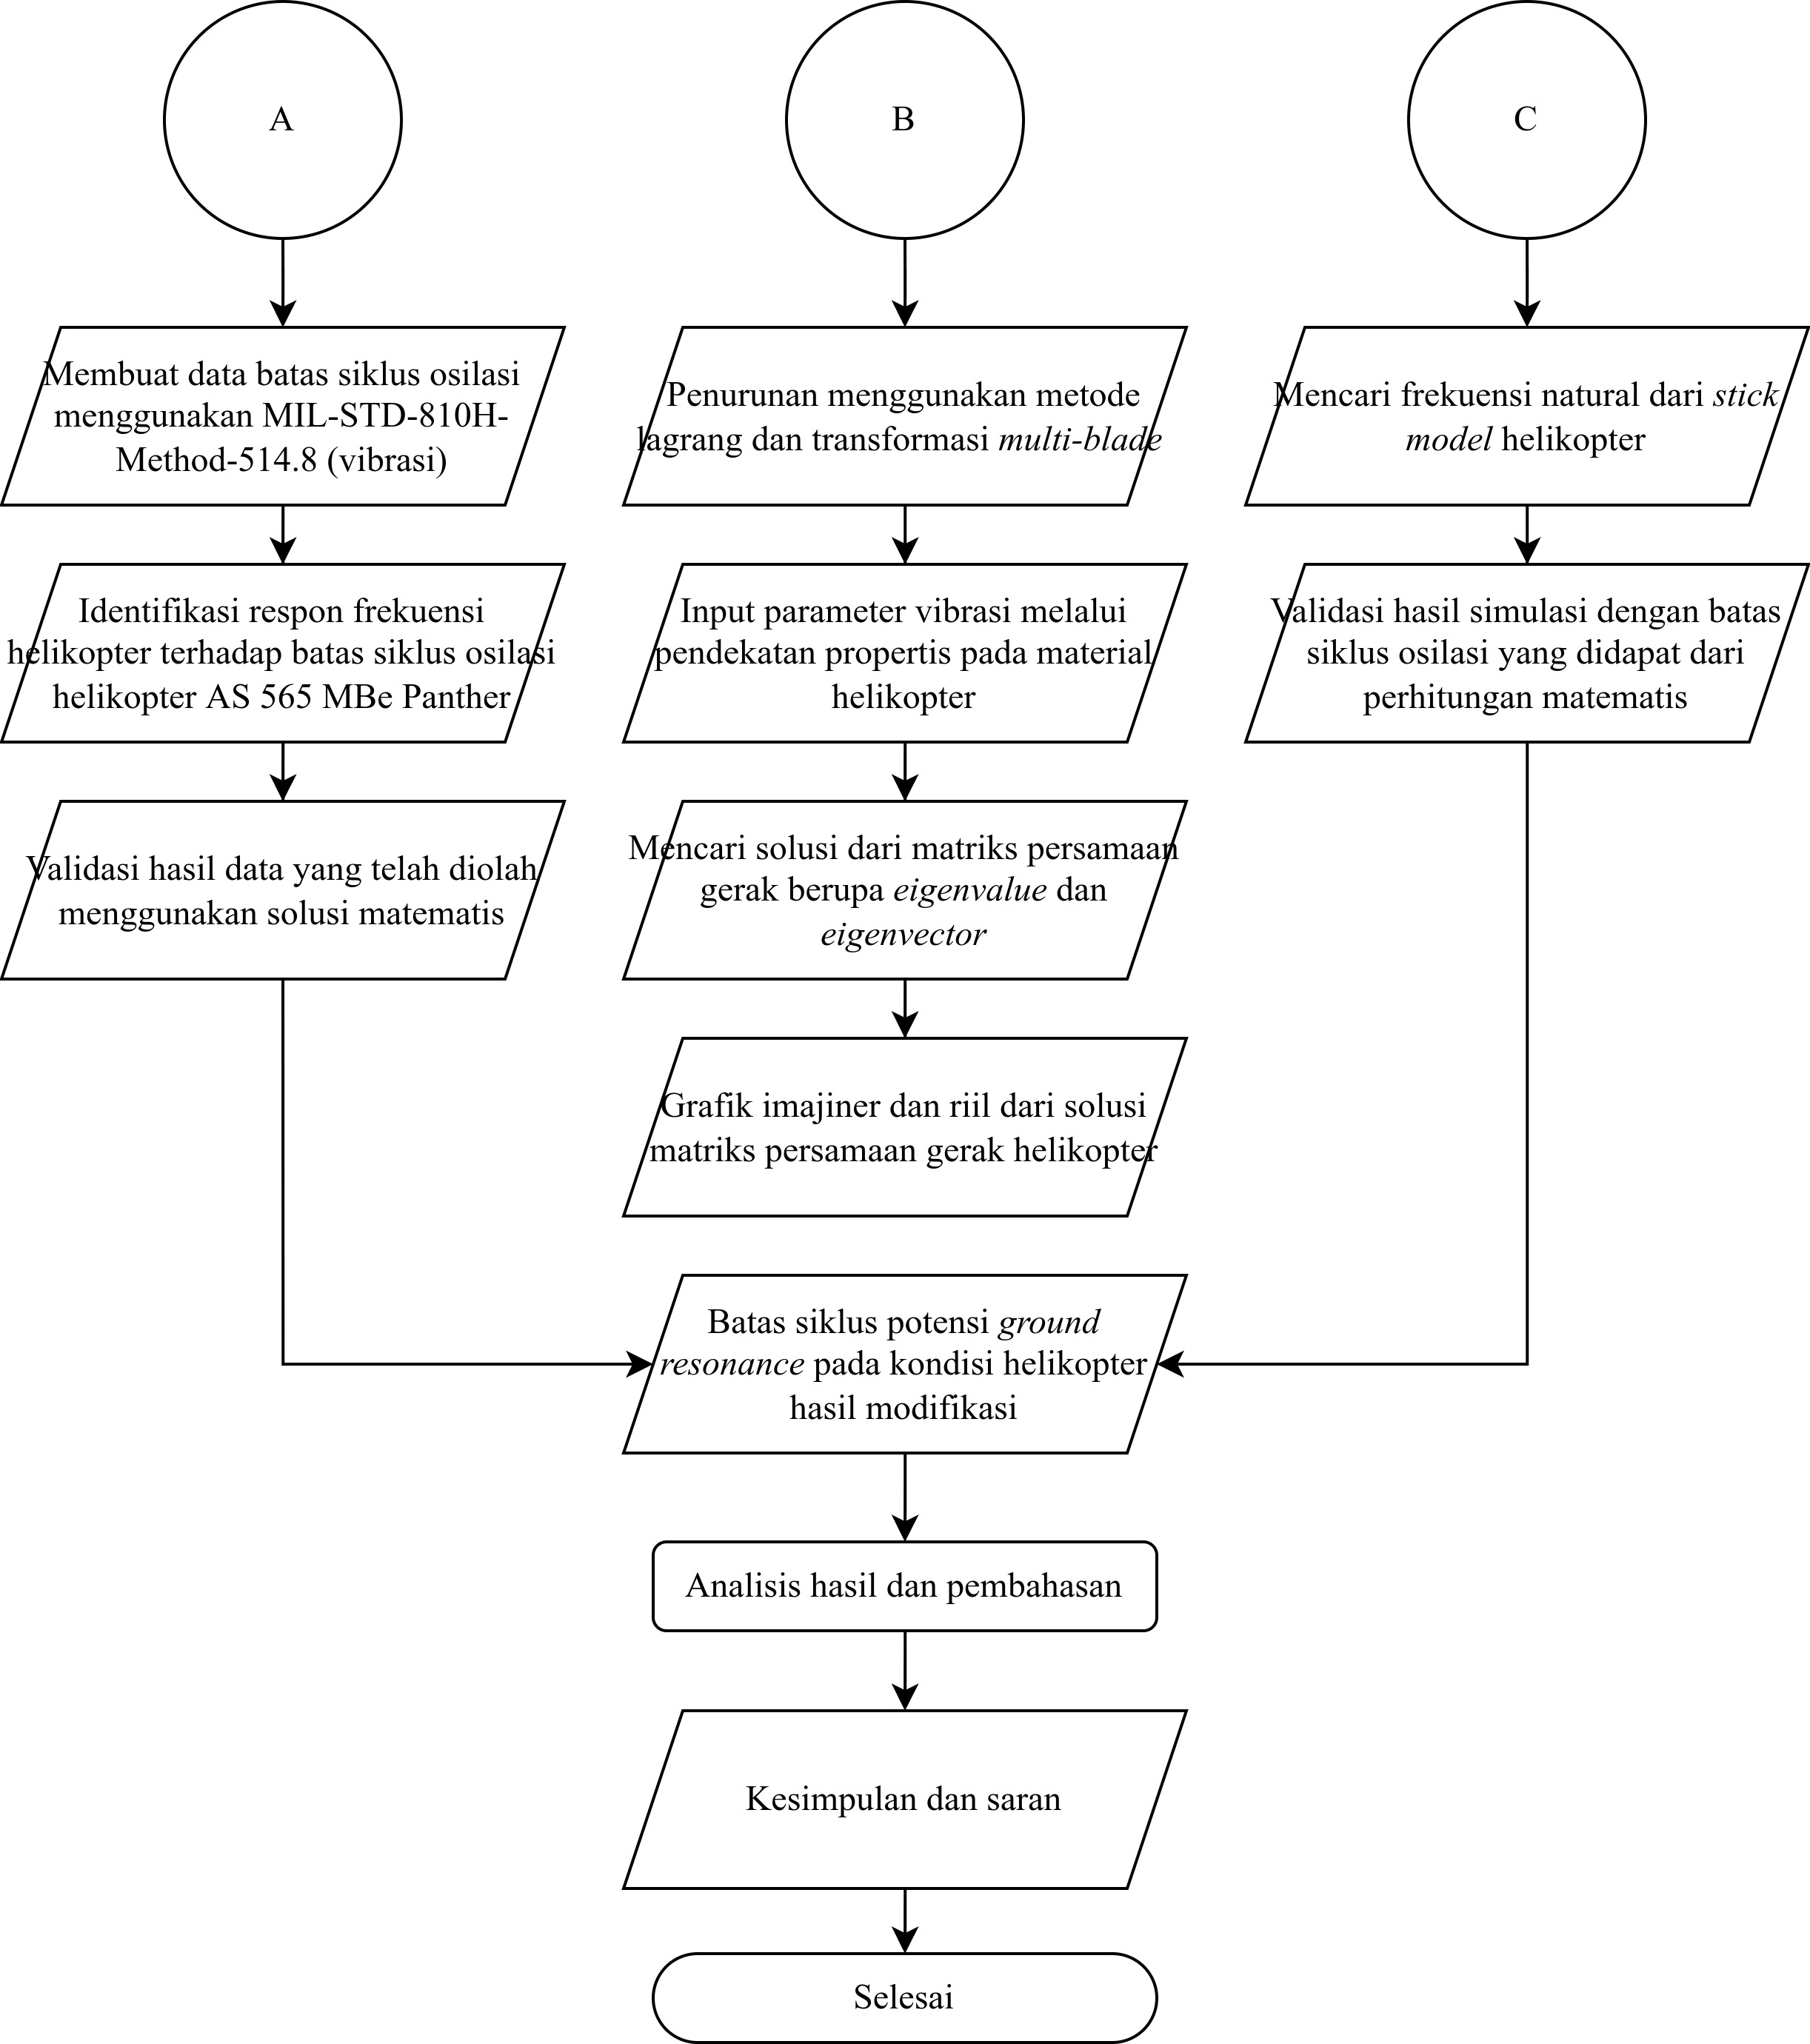
\includegraphics[width=0.95\linewidth]{gambar/TA_flow-Page-2.jpg}
	\caption{Diagram alir pengerjaan Tugas Akhir bagian 2.}
	\label{fig:TA_flow-Page-2.jpg}
\end{figure}

\section{Studi Pustaka}
\label{sec:studipustaka}

Studi pustaka merupakan tahap untuk membaca dan memahami referensi solusi serta metode peneliti sebelumnya berkaitan dengan \textit{ground resonance} pada helikopter. Beberapa referensi yang mendukung terhadap topik ini adalah mengenai metode pengolahan data hasil pengukuran menggunakan MIL-STD-810H-Method-514.8 (vibrasi), perhitungan matematis yang menggunakan konsep dasar dari parameter pegas-peredam-massa, penyelesaian matematis dengan menggunakan lagrang, transformasi \textit{multiblade} matriks, dan solusi eigen dengan bantuan komputasi Matlab. Kemudian referensi lain berupa informasi untuk pemakaian \textit{software} Femap dalam aspek simulasinya.

\section{Pengambilan Data \textit{Ground Test}}
  \label{sec:pengukurandata}

Pengambilan data \textit{ground test} dilakukan dengan mengikuti mekanisme yang telah ditetapkan oleh PTDI. Terdapat 2 pengukuran yang dilakukan, pertama adalah pengukuran terhadap \textit{damping ratio} dari respon helikopter terhadap impuls yang diberikan oleh pilot. Kedua, adalah pengukuran yang didapatkan menggunakan sensor akselerometer yang dipasangkan di beberapa titik pada helikopter.

\subsection{Pengukuran Data Vibrasi pada FTIS}
Pengukuran yang didapatkan dari \textit{Flight Test Instrumentation System} (FTIS) merupakan pengukuran respon gerakan keseluruhan helikopter pada beberapa orientasi gerakan. Respon terhadap impuls lateral serta longitudinal oleh pilot digunakan untuk mengetahui redaman getaran pada struktur helikopter. Nilai \textit{logarithmic decrement} didapatkan dari hasil pengukuran oleh FTIS dengan melihat seberapa cepat amplitudo getaran helikopter teredam sepanjang waktu setelah diberi impuls oleh pilot, nilai ini nantinya akan digunakan untuk menghitung \textit{damping ratio} helikopter. FTIS terletak pada bagian pusat massa helikopter. Karena helikopter dianggap sebagai massa titik yang dapat bergerak pada orientasi 3 dimensi, baik secara getaran translasi ataupun getaran rotasi. Sehingga pada pengukuran ini, nantinya akan didapatkan \textit{output} getaran berupa \textit{roll, pitch, heading, rate of roll, rate of pitch, rate of yaw}, percepatan arah sumbu-x, y, dan z.

\subsection{Pengukuran Data Vibrasi Akselerometer}
Pengukuran vibrasi dengan menggunakan akselerometer dilakukan dibeberapa titik pada helikopter. Konfigurasi mengenai peletakan sensor akselerometer dapat dilihat pada gambar dan tabel berikut.

\begin{figure}[H]
	\centering
	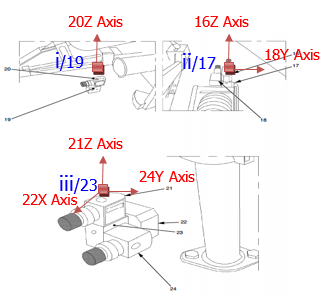
\includegraphics[width=0.6\linewidth]{gambar/peletakan_sensor.png}
	\caption{Peletakan akseleromter pada Helikopter.}
	\label{peletakan_sensor.png}
\end{figure}

\begin{longtable}{|c|c|}
	\caption{Lokasi dan arah akseleromter.}
	\label{tb:lokasiakselero}                        	\\
	\hline
	\textbf{Channel} & \textbf{Lokasi akselerometer} 	\\
	\hline
	1            	 & Kursi pilot (20Z)             	\\
	\hline
	2			     & Bagian luar stik kopilot (16Z)   \\
	\hline
	3				 & Bagian luar stik kopilot	(18Y)   \\
	\hline
	4				 & Frame 9" (21Z)                   \\
	\hline
	5				 & Frame 9" (22X)					\\
	\hline
	6				 & Frame 9" (24Y)					\\
	\hline
\end{longtable}

Kemudian berikut ini merupakan skema Helikopter AS 565 MBe Panther yang digunakan beserta keterangan dimensi dari beberapa arah skema.

\begin{figure}[H]
	\centering
	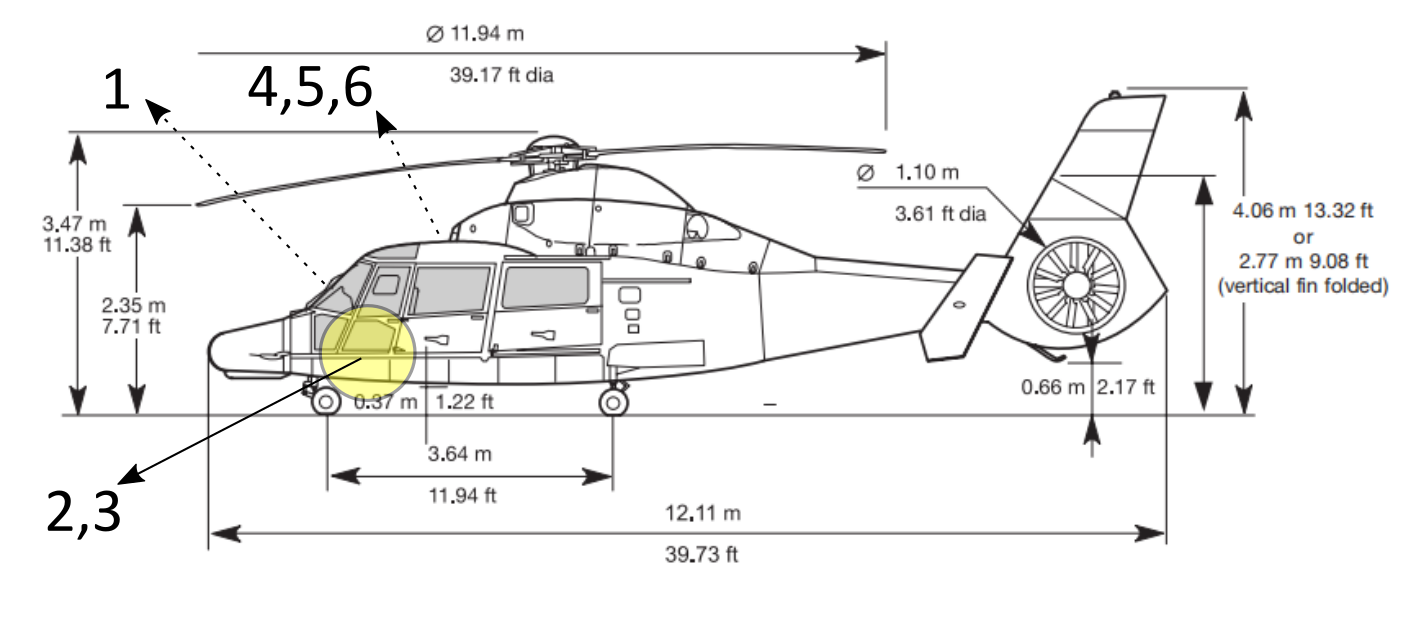
\includegraphics[width=0.8\linewidth]{gambar/tampak_samping.png}
	\caption{Skema penempatan \textit{channel} sensor dan dimensi helikopter AS 565 MBe Panther (tampak samping).}
	\label{tampak_samping.png}
\end{figure}

\begin{figure}[H]
	\centering
	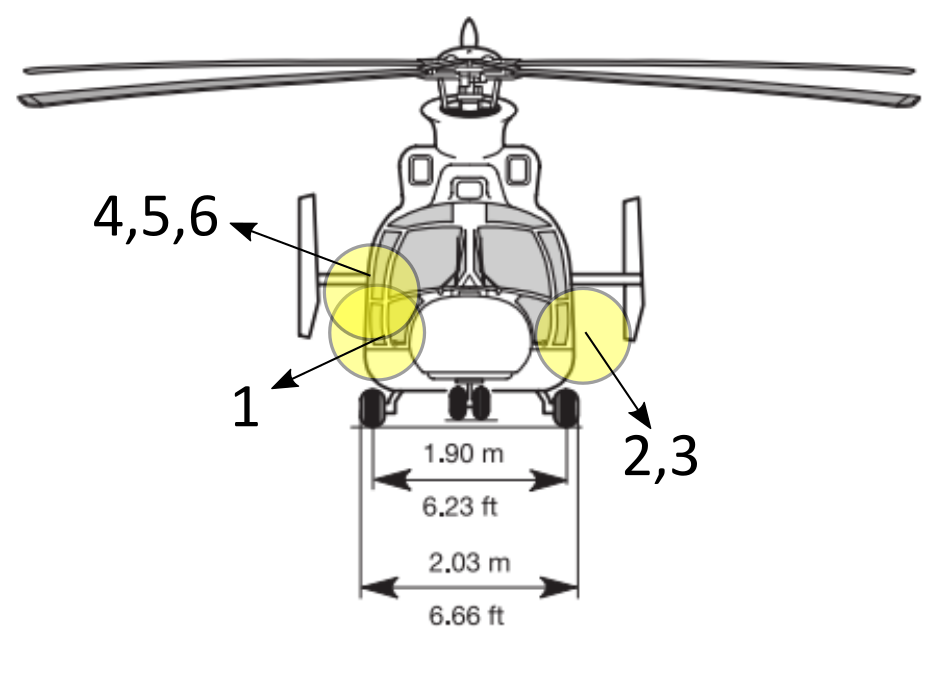
\includegraphics[width=0.6\linewidth]{gambar/tampak_depan.png}
	\caption{Skema penempatan \textit{channel} sensor dan dimensi helikopter AS 565 MBe Panther (tampak depan).}
	\label{tampak_depan.png}
\end{figure}

\begin{figure}[H]
	\centering
	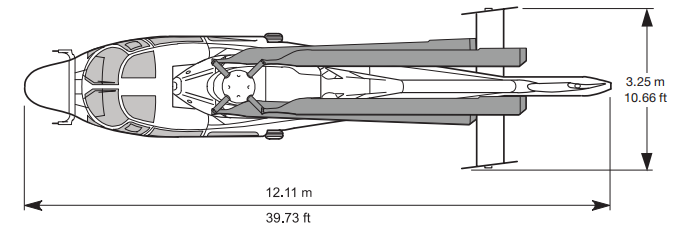
\includegraphics[width=0.75\linewidth]{gambar/tampak_atas.png}
	\caption{Skema penempatan \textit{channel} sensor dan dimensi helikopter AS 565 MBe Panther (tampak atas).}
	\label{tampak_atas.png}
\end{figure}

Tabel \ref{tb:variasilanding} merupakan variasi pada \textit{landing gear absorbers}. Variasi tersebut dilakukan pada bagian ban dan oleo helikopter. Propertis mengenai variasi \textit{landing gear absorbers} ditampilkan pada tabel \ref{tb:propertiskuantitatif}. Selanjutnya pada tabel \ref{tb:variasi_input} memberikan informasi yang berkaitan dengan variasi \textit{input} pada \textit{ground test}. Secara teknis, dalam 1 kondisi pengujian terdapat 12 variasi \textit{input} yang diberikan kepada helikopter.

\begin{table}[H]
	\centering
	\caption{Variasi \textit{Landing gear absorbers.}}
	\label{tb:variasilanding}
	\resizebox{0.7\textwidth}{!}{%
		\begin{tabular}{|c|ccccc|}
			\hline
			\multirow{3}{*}{No} & \multicolumn{5}{c|}{Kondisi pengujian Oleo/Tyre} \\ \cline{2-6} 
			& \multicolumn{1}{c|}{Bagian Depan} & \multicolumn{2}{c|}{Bagian Kiri} & \multicolumn{2}{c|}{Bagian Kanan} \\ \cline{2-6} 
			& \multicolumn{1}{c|}{Oleo/Tyre} & \multicolumn{1}{c|}{Oleo} & \multicolumn{1}{c|}{Tyre} & \multicolumn{1}{c|}{Oleo} & Tyre \\ \hline
			1 & \multicolumn{1}{c|}{Nominal/Nominal} & \multicolumn{1}{c|}{Nominal} & \multicolumn{1}{c|}{Nominal} & \multicolumn{1}{c|}{Nominal} & Nominal \\ \hline
			2 & \multicolumn{1}{c|}{Nominal/Nominal} & \multicolumn{1}{c|}{High} & \multicolumn{1}{c|}{High} & \multicolumn{1}{c|}{Nominal} & Nominal \\ \hline
			3 & \multicolumn{1}{c|}{Nominal/Nominal} & \multicolumn{1}{c|}{Nominal} & \multicolumn{1}{c|}{Nominal} & \multicolumn{1}{c|}{High} & High \\ \hline
			4 & \multicolumn{1}{c|}{Nominal/Nominal} & \multicolumn{1}{c|}{Nominal} & \multicolumn{1}{c|}{Nominal} & \multicolumn{1}{c|}{Low} & Low \\ \hline
			5 & \multicolumn{1}{c|}{Nominal/Nominal} & \multicolumn{1}{c|}{Low} & \multicolumn{1}{c|}{Low} & \multicolumn{1}{c|}{Nominal} & Nominal \\ \hline
			6 & \multicolumn{1}{c|}{Nominal/Nominal} & \multicolumn{1}{c|}{High} & \multicolumn{1}{c|}{High} & \multicolumn{1}{c|}{High} & High \\ \hline
			7 & \multicolumn{1}{c|}{Nominal/Nominal} & \multicolumn{1}{c|}{Low} & \multicolumn{1}{c|}{Low} & \multicolumn{1}{c|}{Low} & Low \\ \hline
			8 & \multicolumn{1}{c|}{Nominal/Nominal} & \multicolumn{1}{c|}{High} & \multicolumn{1}{c|}{High} & \multicolumn{1}{c|}{Low} & Low \\ \hline
			9 & \multicolumn{1}{c|}{Nominal/Nominal} & \multicolumn{1}{c|}{Low} & \multicolumn{1}{c|}{Low} & \multicolumn{1}{c|}{High} & High \\ \hline
			10 & \multicolumn{1}{c|}{Nominal/Nominal} & \multicolumn{1}{c|}{High} & \multicolumn{1}{c|}{High} & \multicolumn{1}{c|}{Nominal} & High \\ \hline
			11 & \multicolumn{1}{c|}{Nominal/Nominal} & \multicolumn{1}{c|}{High} & \multicolumn{1}{c|}{High} & \multicolumn{1}{c|}{Low} & High \\ \hline
		\end{tabular}%
	}
\end{table}

\begin{table}[h]
	\centering
	\caption{Propertis kuantitatif variasi \textit{landing gear absorbers} pada ban dan oleo helikopter.}
	\label{tb:propertiskuantitatif}
	\resizebox{0.75\textwidth}{!}{%
		\begin{tabular}{|c|c|c|l|}
			\hline
			\multirow{3}{*}{NLG} & \multirow{2}{*}{Oleo} & \multirow{2}{*}{Nominal} & Hydraulic: 10 bar (145 psi) \\ \cline{4-4} 
			&  &  & Nitrogen 30$^o$C=42 bar(psi) \\ \cline{2-4} 
			& Tyre & Nominal & 5.5 bar (79.7 psi) \\ \hline
			\multirow{9}{*}{MLG} & \multirow{6}{*}{Oleo} & \multirow{2}{*}{Low} & Hydraulic: 10 bar (145 psi) \\ \cline{4-4} 
			&  &  & Nitrogen 15oC: HP=49.0 bar (711 psi) LP=4.0 bar (59.0 psi) \\ \cline{3-4} 
			&  & \multirow{2}{*}{Nominal} & Hydraulic: 10 bar (145 psi) \\ \cline{4-4} 
			&  &  & Nitrogen 30$^o$C: HP=51.5 bar (747 psi) LP=4.2 bar (61 psi) \\ \cline{3-4} 
			&  & \multirow{2}{*}{High} & Hydraulic: 10 bar (145 psi) \\ \cline{4-4} 
			&  &  & Nitrogen 45$^o$C: HP=54.0 bar (783 psi) LP=4.4 bar (63.82 psi) \\ \cline{2-4} 
			& \multirow{3}{*}{Tyre} & Low & 8.48 bar (123 psi) \\ \cline{3-4} 
			&  & Nominal & 10.8 bar (156.6 psi) \\ \cline{3-4} 
			&  & High & 13.1 bar (190 psi) \\ \hline
		\end{tabular}%
	}
\end{table}

\begin{table}[h]
	\centering
	\caption{Variasi \textit{input} pada ground test Helikopter.}
	\label{tb:variasi_input}
	\resizebox{0.75\textwidth}{!}{%
		\begin{tabular}{|c|c|c|c|c|}
			\hline
			No & SAS & Power & Input Control & Name of Sequence \\ \hline
			1 & \multirow{6}{*}{OFF} & Ground Idle & Longitudinal & FILO \\ \cline{1-1} \cline{3-5} 
			2 &  & Ground Idle & Lateral & FILA \\ \cline{1-1} \cline{3-5} 
			3 &  & Flight Idle (on Ground) & Longitudinal & FFLO \\ \cline{1-1} \cline{3-5} 
			4 &  & Flight Idle (on Ground) & Lateral & FFLA \\ \cline{1-1} \cline{3-5} 
			5 &  & Flight Idle (Light on Wheel) & Longitudinal & FLLO \\ \cline{1-1} \cline{3-5} 
			6 &  & Flight Idle (Light on Wheel) & Lateral & FLLA \\ \hline
			7 & \multirow{6}{*}{ON} & Ground Idle & Longitudinal & NILO \\ \cline{1-1} \cline{3-5} 
			8 &  & Ground Idle & Lateral & NILA \\ \cline{1-1} \cline{3-5} 
			9 &  & Flight Idle (on Ground) & Longitudinal & NFLO \\ \cline{1-1} \cline{3-5} 
			10 &  & Flight Idle (on Ground) & Lateral & NFLA \\ \cline{1-1} \cline{3-5} 
			11 &  & Flight Idle (Light on Wheel) & Longitudinal & NLLO \\ \cline{1-1} \cline{3-5} 
			12 &  & Flight Idle (Light on Wheel) & Lateral & NLLA \\ \hline
		\end{tabular}%
	}
\end{table}

Semua data yang didapatkan pada hasil pengukuran \textit{damping ratio} dan vibrasi oleh akselerometer selanjutnya akan diolah dan dianalisis apakah helikopter AS 565 MBe Panther hasil modifikasi tersebut berpotensi mengalami fenomena \textit{ground resonance}. Sehingga helikopter dapat dikatakan aman untuk dapat digunakan sebagaimana kegunaannya setelah dimodifikasi. Kemudian, data vibrasi pada akselerometer akan dimasukkan pada batas siklus osilasi sesuai dengan acuan yang terdapat pada MIL-STD-810H-Method-514.8 (vibrasi).

\begin{table}[]
	\centering
	\caption{Tabel acuan MIL-STD-810H-Method-514.8 untuk menghitung batas osilasi yang dimiliki oleh helikopter.}
	\label{tb:MIL-STD}
	\resizebox{\textwidth}{!}{%
		\begin{tabular}{|cccc|}
			\hline
			\multicolumn{1}{|c|}{Materiel} & \multicolumn{1}{c|}{Random Levels} & \multicolumn{1}{c|}{\begin{tabular}[c]{@{}c@{}}Source Frequency ($f_x$)\\ Range (Hz)\end{tabular}} & \begin{tabular}[c]{@{}c@{}}Peak Acceleration ($A_x$) \\ at $f_x$ (Gravity Units (g))\end{tabular} \\ \hline
			\multicolumn{1}{|c|}{\multirow{5}{*}{General}} & \multicolumn{1}{c|}{$W_o = 0.0010 g^2/Hz$} & \multicolumn{1}{c|}{$3 to \leq 10$} & 0.7/(10.70-$f_x$) \\ \cline{2-4} 
			\multicolumn{1}{|c|}{} & \multicolumn{1}{c|}{$W_1 = 0.010 g^2/Hz$} & \multicolumn{1}{c|}{$>10$ to $25$} & 0.10 $f_x$ \\ \cline{2-4} 
			\multicolumn{1}{|c|}{} & \multicolumn{1}{c|}{\multirow{3}{*}{$f_1=500 Hz$}} & \multicolumn{1}{c|}{25 to 40} & 2.5 \\ \cline{3-4} 
			\multicolumn{1}{|c|}{} & \multicolumn{1}{c|}{} & \multicolumn{1}{c|}{40 to 50} & 6.50 - 0.1 $f_x$ \\ \cline{3-4} 
			\multicolumn{1}{|c|}{} & \multicolumn{1}{c|}{} & \multicolumn{1}{c|}{50 to 500} & 1.5 \\ \hline
			\multicolumn{4}{|c|}{Main Rotor Frequencies (Hz)} \\ \hline
			\multicolumn{2}{|c|}{$f_1$ = 1P} & \multicolumn{2}{c|}{Fundamental} \\ \hline
			\multicolumn{2}{|c|}{$f_2$ = n*1P} & \multicolumn{2}{c|}{blade passage (BP)} \\ \hline
			\multicolumn{2}{|c|}{$f_3 = 2f_2$} & \multicolumn{2}{c|}{$2^{nd}$ harmonic} \\ \hline
			\multicolumn{2}{|c|}{$f_4 = 3f_2$} & \multicolumn{2}{c|}{$3^{rd}$ harmonic} \\ \hline
		\end{tabular}%
	}
\end{table}

\section{Pemodelan pada Femap}
	\label{sec:femap}
\subsection{Skema Pemodelan}
Dalam mencari solusi yang secara tepat merepresentasikan batas siklus osilasi pada perhitungan matematis. Berdasarkan referensi yang telah didapatkan, diperlukan langkah awal membuat skema pemodelan sederhana yang selanjutnya akan membantu untuk mendefinisikan posisi pusat massa dari masing-masing rotor pada helikopter. Skema pemodelan ini berdasarkan pada gambar \ref{tampak_atas.png} untuk menggambar bagian helikopter pada bagian tampak atas. Sedangkan gambar \ref{tampak_samping.png}. Skema gambar menggunakan bantuan \textit{software} desain Inkscape untuk memberikan bentuk \textit{node} pada kerangka yang helikopter yang ingin digambar. Berikut ini merupakan skema kerangka helikopter untuk memodelkan helikopter dengan bentuk yang sederhana agar nantinya dapat diolah menggunakan prinsip elemen hingga (\textit{finite element}) pada \textit{software} FEMAP.

\begin{figure}[H]
	\centering
	\includegraphics[width=\linewidth]{gambar/rancangan_skema.png}
	\caption{Skema pemodelan helikopter untuk bagian samping, atas, dan bawah.}
	\label{fig:skema_model}
\end{figure}

Koordinat pada helikopter didapatkan dengan menggunakan dimensi yang mendekati ukuran sebenarnya dari helikopter. Oleh karena itu pada gambar \ref{fig:skema_model} digunakan bayangan kerangka helikopter yang sebenarnya dari AS 565 MBe Panther. Rasio yang dimiliki pada skema gambar tersebut adalah 0.0778m/mm, yang artinya dalam setiap panjang 1mm pada gambar, mewakili 0.0778 meter pada dimensi helikopter yang sebenarnya.

\subsection{Penentuan Koordinat}

Selanjutnya, pada gambar \ref{fig:skema_model} akan didefinisikan titik-titik yang nantinya akan menjadi \textit{node} pada kerangka helikopter. Titik-titik tersebut akan didefinisikan dalam koordinat kartesian dalam sumbu-x,y, dan z. Titik 2s', 2s dan 3s' akan menjadi titik diberikannya gaya luar untuk simulasi pada FEMAP. Hal ini dikarenakan pada titik tersebut terdapat sensor akselerometer.


\begin{table}[h]
	\centering
	\caption{Koordinat masing-masing tanda pada titik dalam 3 dimensi.}
	\label{tb:koordinat}
	\resizebox{0.93\textwidth}{!}{%
		\begin{tabular}{|
				>{\columncolor[HTML]{FFCCC9}}c |
				>{\columncolor[HTML]{FFCE93}}c |ccc|
				>{\columncolor[HTML]{FFCCC9}}c |
				>{\columncolor[HTML]{FFCE93}}c |ccc|}
			\hline
			\cellcolor[HTML]{FFCCC9} & \cellcolor[HTML]{FFCE93} & \multicolumn{3}{c|}{Koordinat (m)} & \cellcolor[HTML]{FFCCC9} & \cellcolor[HTML]{FFCE93} & \multicolumn{3}{c|}{Koordinat (m)} \\ \cline{3-5} \cline{8-10} 
			\multirow{-2}{*}{\cellcolor[HTML]{FFCCC9}ID} & \multirow{-2}{*}{\cellcolor[HTML]{FFCE93}Mark} & \multicolumn{1}{c|}{x} & \multicolumn{1}{c|}{y} & z & \multirow{-2}{*}{\cellcolor[HTML]{FFCCC9}ID} & \multirow{-2}{*}{\cellcolor[HTML]{FFCE93}Mark} & \multicolumn{1}{c|}{x} & \multicolumn{1}{c|}{y} & z \\ \hline
			1 & 10s & \multicolumn{1}{c|}{8.4295} & \multicolumn{1}{c|}{0.4676} & 0.3466 & 17 & 4s & \multicolumn{1}{c|}{4.3831} & \multicolumn{1}{c|}{-0.1945} & -0.4085 \\ \hline
			2 & 11s & \multicolumn{1}{c|}{8.8695} & \multicolumn{1}{c|}{0.4806} & 0.3466 & 18 & 4s' & \multicolumn{1}{c|}{4.3831} & \multicolumn{1}{c|}{-0.1945} & 1.1987 \\ \hline
			3 & 12s & \multicolumn{1}{c|}{10.2371} & \multicolumn{1}{c|}{0.6235} & 0.3466 & 19 & 5a & \multicolumn{1}{c|}{1.4013} & \multicolumn{1}{c|}{0.9972} & -0.0374 \\ \hline
			4 & 13s & \multicolumn{1}{c|}{10.2087} & \multicolumn{1}{c|}{1.5276} & 0.3466 & 20 & 5a' & \multicolumn{1}{c|}{1.4013} & \multicolumn{1}{c|}{0.9972} & 0.7295 \\ \hline
			5 & 14s & \multicolumn{1}{c|}{10.9654} & \multicolumn{1}{c|}{3.0033} & 0.3466 & 21 & 5s & \multicolumn{1}{c|}{1.6449} & \multicolumn{1}{c|}{0.9972} & -0.32144 \\ \hline
			6 & 15s & \multicolumn{1}{c|}{11.1567} & \multicolumn{1}{c|}{0.8293} & 0.3466 & 22 & 5s' & \multicolumn{1}{c|}{1.6449} & \multicolumn{1}{c|}{0.9972} & 1.0146 \\ \hline
			7 & 1a & \multicolumn{1}{c|}{3.0017} & \multicolumn{1}{c|}{1.739} & 0.7762 & 23 & 6s & \multicolumn{1}{c|}{2.5934} & \multicolumn{1}{c|}{0.9972} & -0.5704 \\ \hline
			8 & 1a' & \multicolumn{1}{c|}{3.0017} & \multicolumn{1}{c|}{1.739} & -0.0801 & 24 & 7a & \multicolumn{1}{c|}{8.8695} & \multicolumn{1}{c|}{0.4806} & 1.6486 \\ \hline
			9 & 1s & \multicolumn{1}{c|}{0} & \multicolumn{1}{c|}{0} & 0 & 25 & 7a' & \multicolumn{1}{c|}{8.8695} & \multicolumn{1}{c|}{0.4806} & -0.9553 \\ \hline
			10 & 1s' & \multicolumn{1}{c|}{0} & \multicolumn{1}{c|}{0} & 0.6932 & 26 & 7s & \multicolumn{1}{c|}{4.3831} & \multicolumn{1}{c|}{0.9972} & -0.4707 \\ \hline
			11 & 2a' & \multicolumn{1}{c|}{5.3859} & \multicolumn{1}{c|}{1.739} & 0.681 & 27 & 8s & \multicolumn{1}{c|}{2.9028} & \multicolumn{1}{c|}{1.739} & -0.5704 \\ \hline
			12 & 2a & \multicolumn{1}{c|}{5.3859} & \multicolumn{1}{c|}{1.739} & 0.0128 & 28 & 8s' & \multicolumn{1}{c|}{2.9028} & \multicolumn{1}{c|}{1.739} & 1.2081 \\ \hline
			13 & 2s & \multicolumn{1}{c|}{1.019} & \multicolumn{1}{c|}{-0.1945} & -0.4085 & 29 & 9s & \multicolumn{1}{c|}{4.8087} & \multicolumn{1}{c|}{1.739} & -0.4707 \\ \hline
			14 & 2s' & \multicolumn{1}{c|}{1.019} & \multicolumn{1}{c|}{-0.1945} & 1.1987 & 30 & 9s' & \multicolumn{1}{c|}{4.8087} & \multicolumn{1}{c|}{1.739} & 1.1639 \\ \hline
			15 & 3s & \multicolumn{1}{c|}{2.6192} & \multicolumn{1}{c|}{-0.1945} & -0.4085 & 31 & 6s' & \multicolumn{1}{c|}{2.5934} & \multicolumn{1}{c|}{0.9972} & 1.2081 \\ \hline
			16 & 3s' & \multicolumn{1}{c|}{2.6192} & \multicolumn{1}{c|}{-0.1945} & 1.1987 & 32 & 7s' & \multicolumn{1}{c|}{4.3831} & \multicolumn{1}{c|}{0.9972} & 1.1639 \\ \hline
		\end{tabular}%
	}
\end{table}

Tabel \ref{tb:koordinat} dan \ref{tb:koordinat-2} merupakan koordinat yang didefinisikan dengan titik acuan berada pada 1s, sehingga titik 1s didefinsikan dengan koordinat x,y, dan z beruturut-turut, 0, 0, dan 0. Setelah koordinat ditentukan, maka pada tahap selanjutnya adalah melakukan pemodelan pada FEMAP untuk selanjutnya nanti akan dilakukan analisis menggunakan nilai eigen untuk mencari \textit{mode shape} pada helikopter. Informasi mengenai \textit{mode shape} ini nantinya akan digunakan untuk memberikan gambaran bahwa helikopter akan memiliki respon sedemikian rupa untuk dapat menjelaskan fenomena \textit{ground resonance} yang berpotensi terjadi pada helikopter.